\clearpage{\pagestyle{empty}\cleardoublepage}

\chapter{Final results}\label{chap:results}

Through Chapters~\ref{chap:vlq},~\ref{chap:wbx} and~\ref{chap:htx}
we presented the strategy adopted for the searches of vector-like
top partners in the single lepton channel and implemented into
two complementary analyses: the \wbx\ and the \htx\ analyses.
Each of these analyses is probing a different
area of the two-dimensional plane (described in Section~\ref{sec:strategy}) 
defined in order to perform
a model-independent scan of the three possible decay channels BR 
mixing phase space.
In this chapter we are going to illustrate how the results
obtained by the individual analyses (Sections~\ref{sec:wbxRES} 
and~\ref{sec:htxRES}) perform when the search channels are
combined (Section~\ref{sec:results_comb}).
In Section~\ref{sec:coverage} we compare
the coverage of the BRs two-dimensional
mixing plane by the four quasi-model independent
searches for vector-like quarks performed
by the Exotics group.


\section{Combination of the \wbx\ and \htx\ analyses}\label{sec:results_comb}

As the \wbx\ and the \htx\ analyses do not overlap
thanks to the orthogonality requirements (rejection of
events with $\geq$ 6 jets and $\geq$ 3 \btag ged jets
in the \wbx\ analysis, rejection of events with $H_T>700~\gev$
in the \chii\ channel of the \htx\ analysis), it is possible
to obtain a fully combined result. Figure~\ref{fig:searchchan}
reports the final search channels to be used.

\begin{figure}[h!tb]\begin{center}
	\subfigure[]{\label{fig:htx2}
%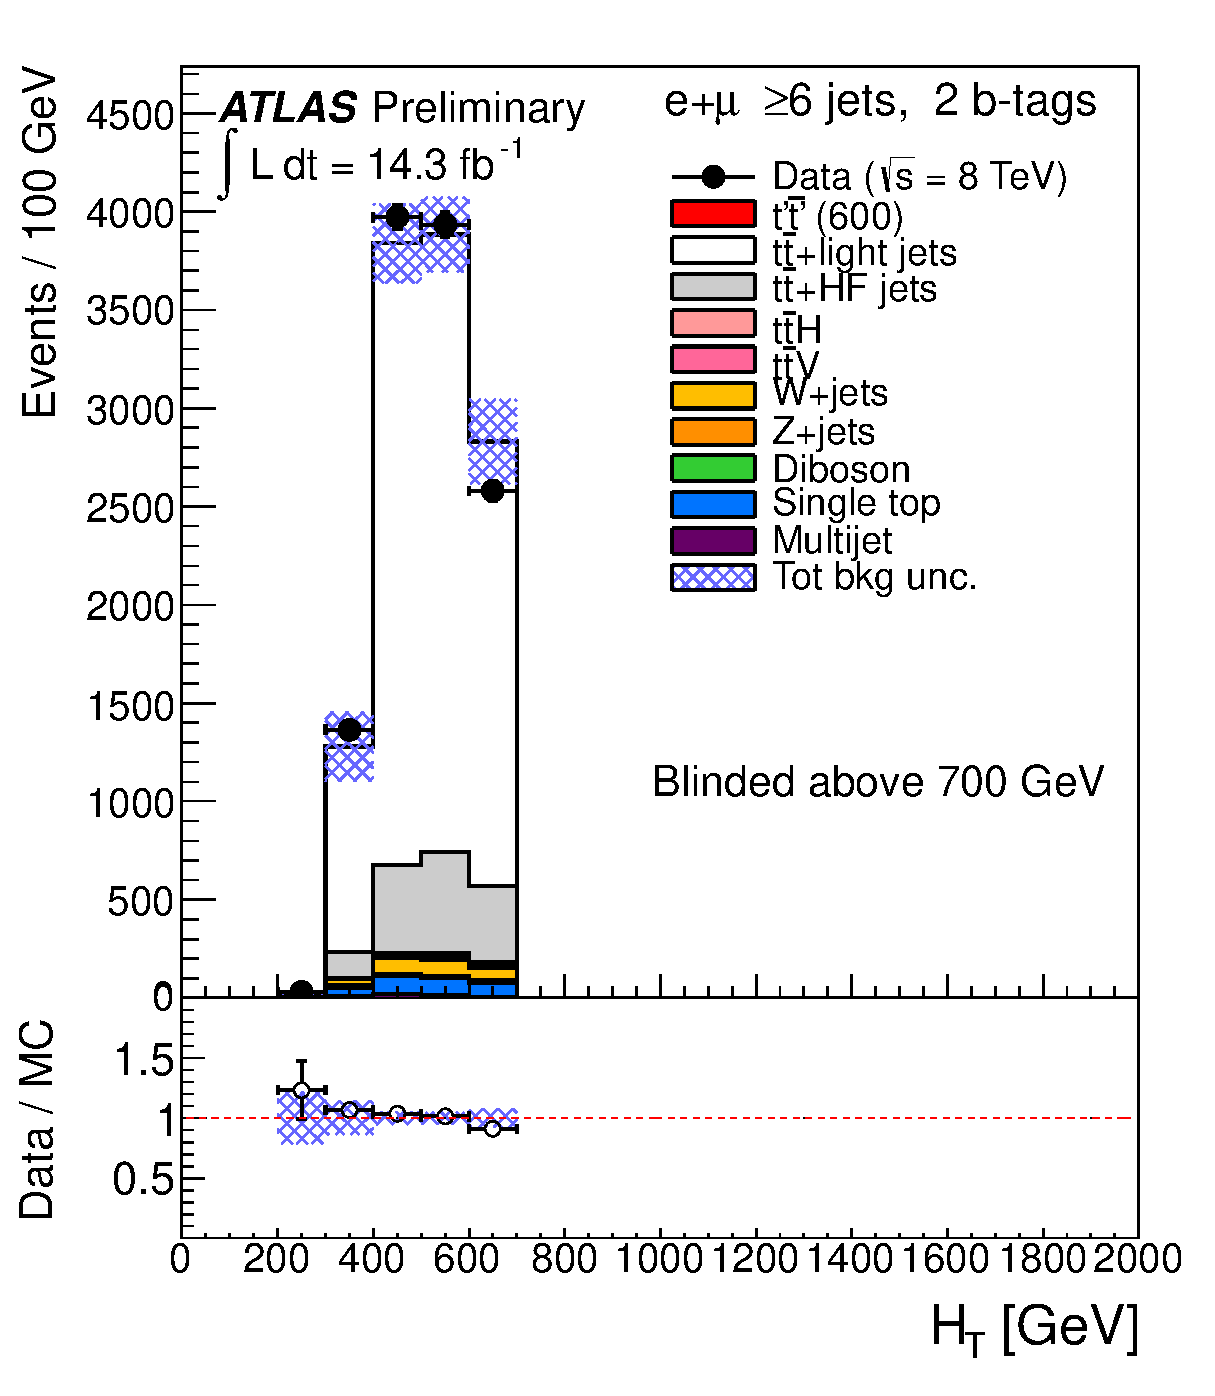
\includegraphics[width=0.45\textwidth]{htx_analysis_14ifb/figures/final/HTAll_6jetin2btagex_ELEMUON.eps}}
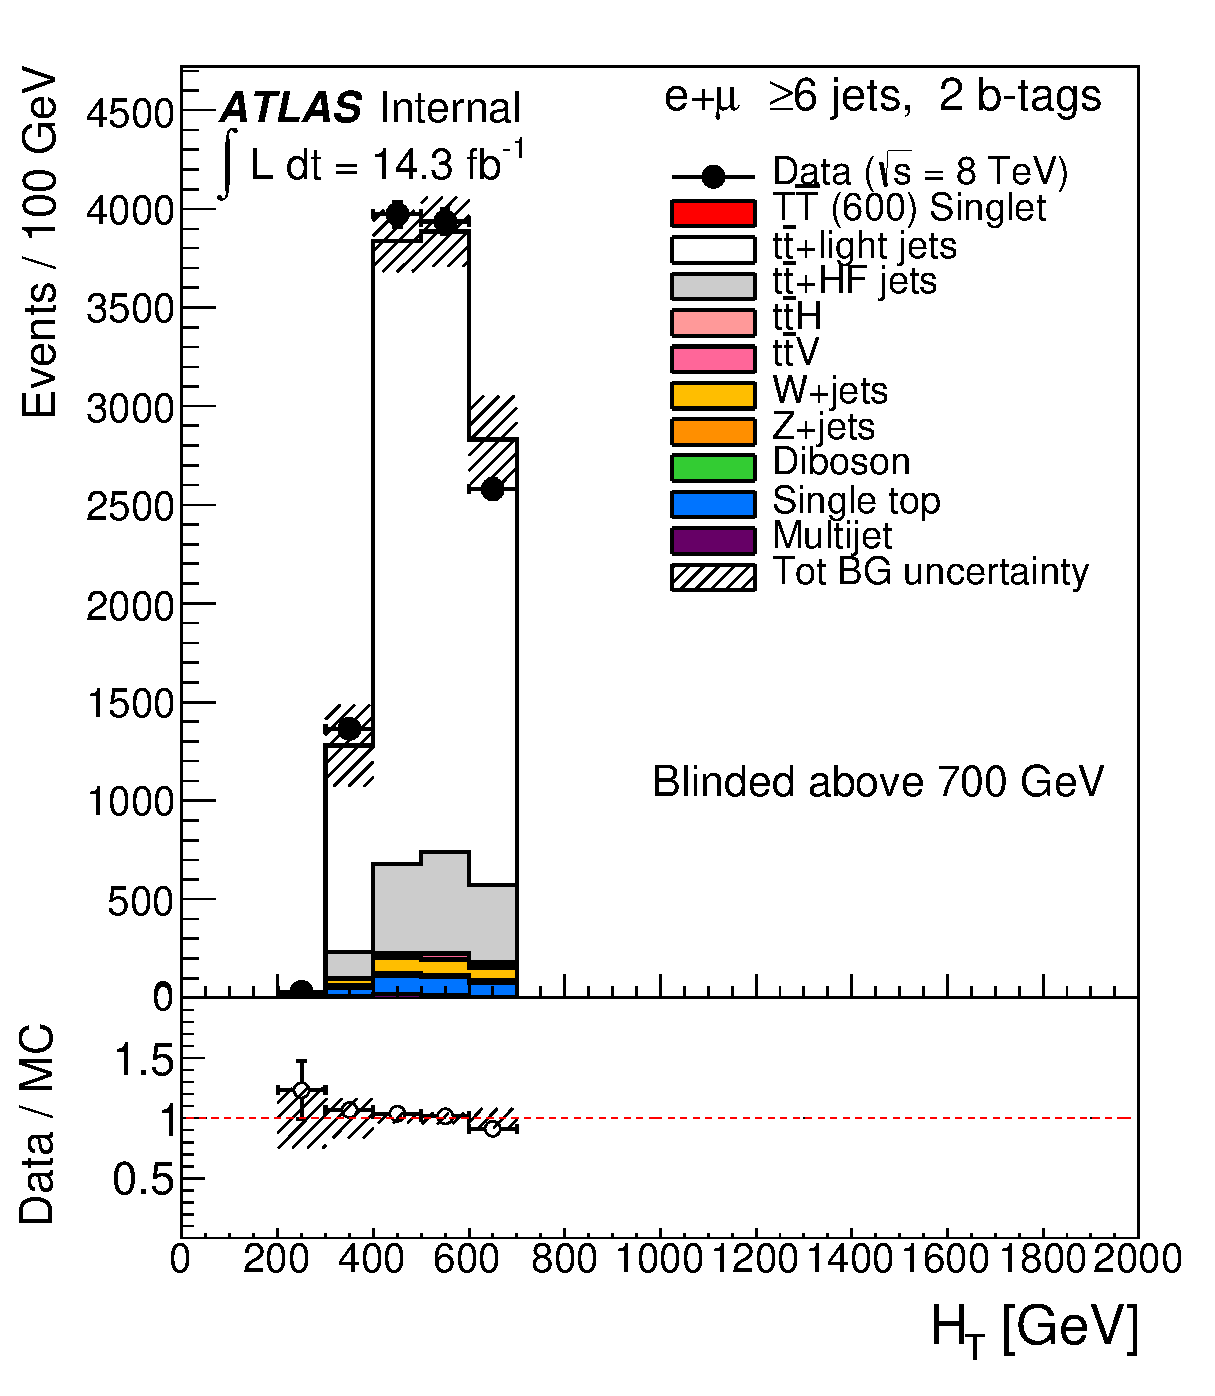
\includegraphics[width=0.45\textwidth]{results/figures/THESIS_c8_signal/HTAll_6jetin2btagex_ELEMUON.eps}}
	\subfigure[]{\label{fig:htx3}
%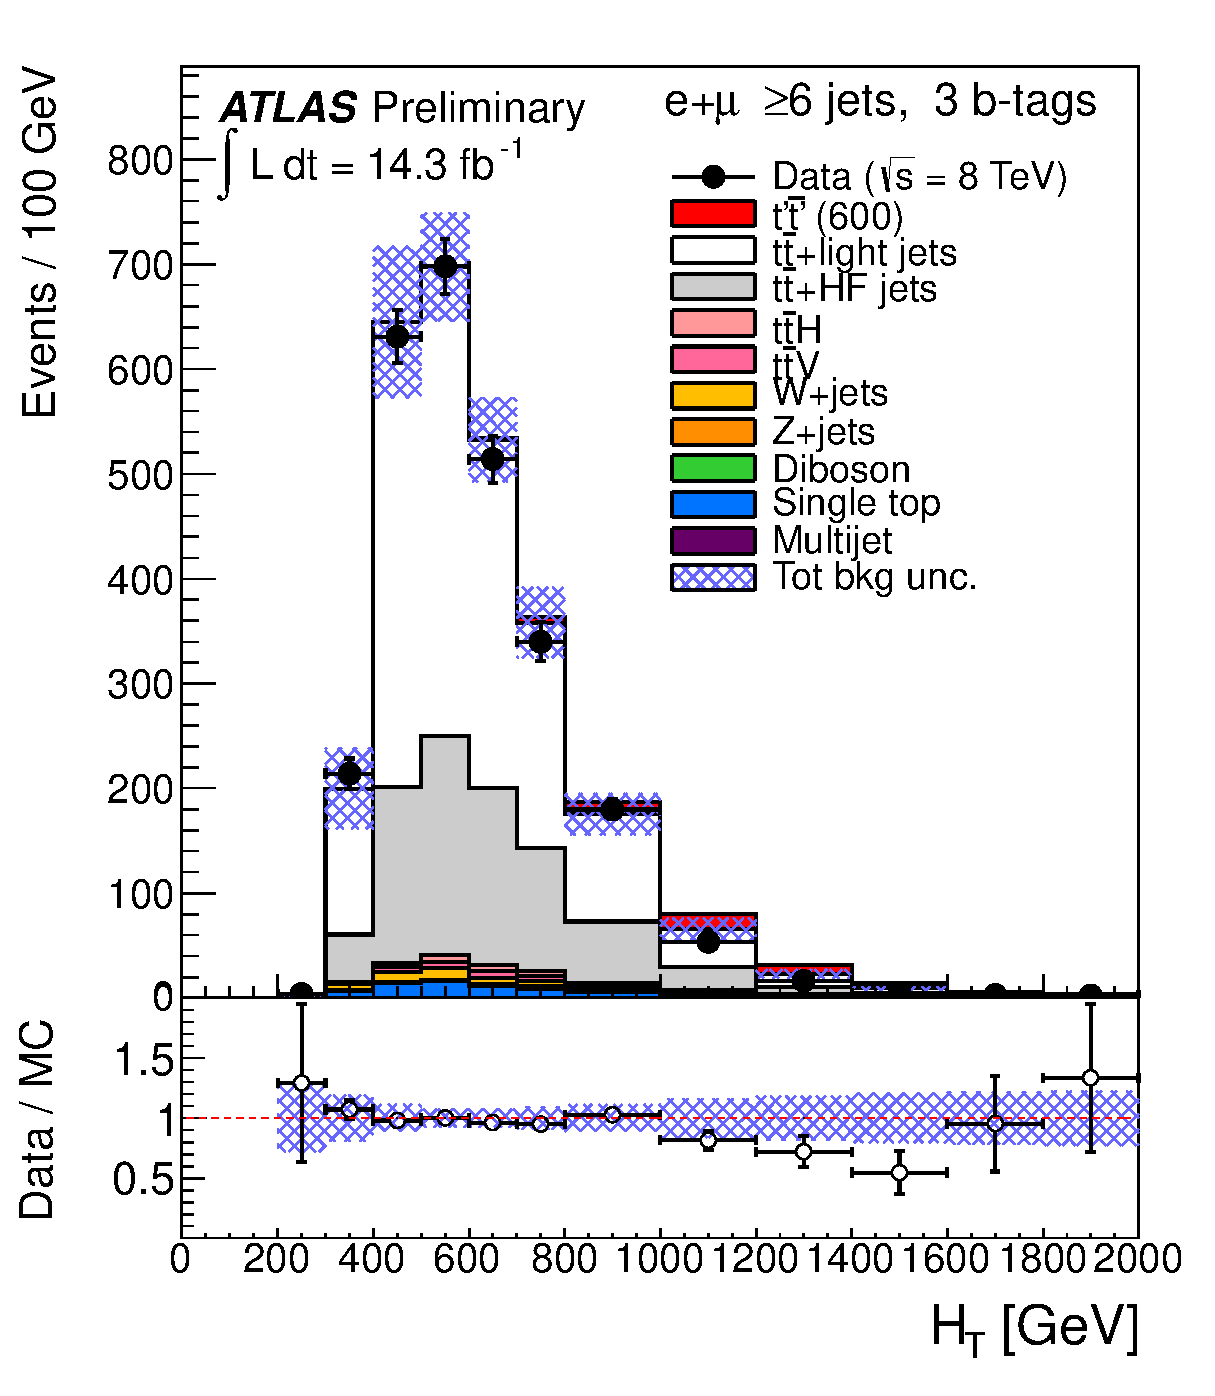
\includegraphics[width=0.45\textwidth]{htx_analysis_14ifb/figures/final/HTAll_6jetin3btagex_ELEMUON.eps}}
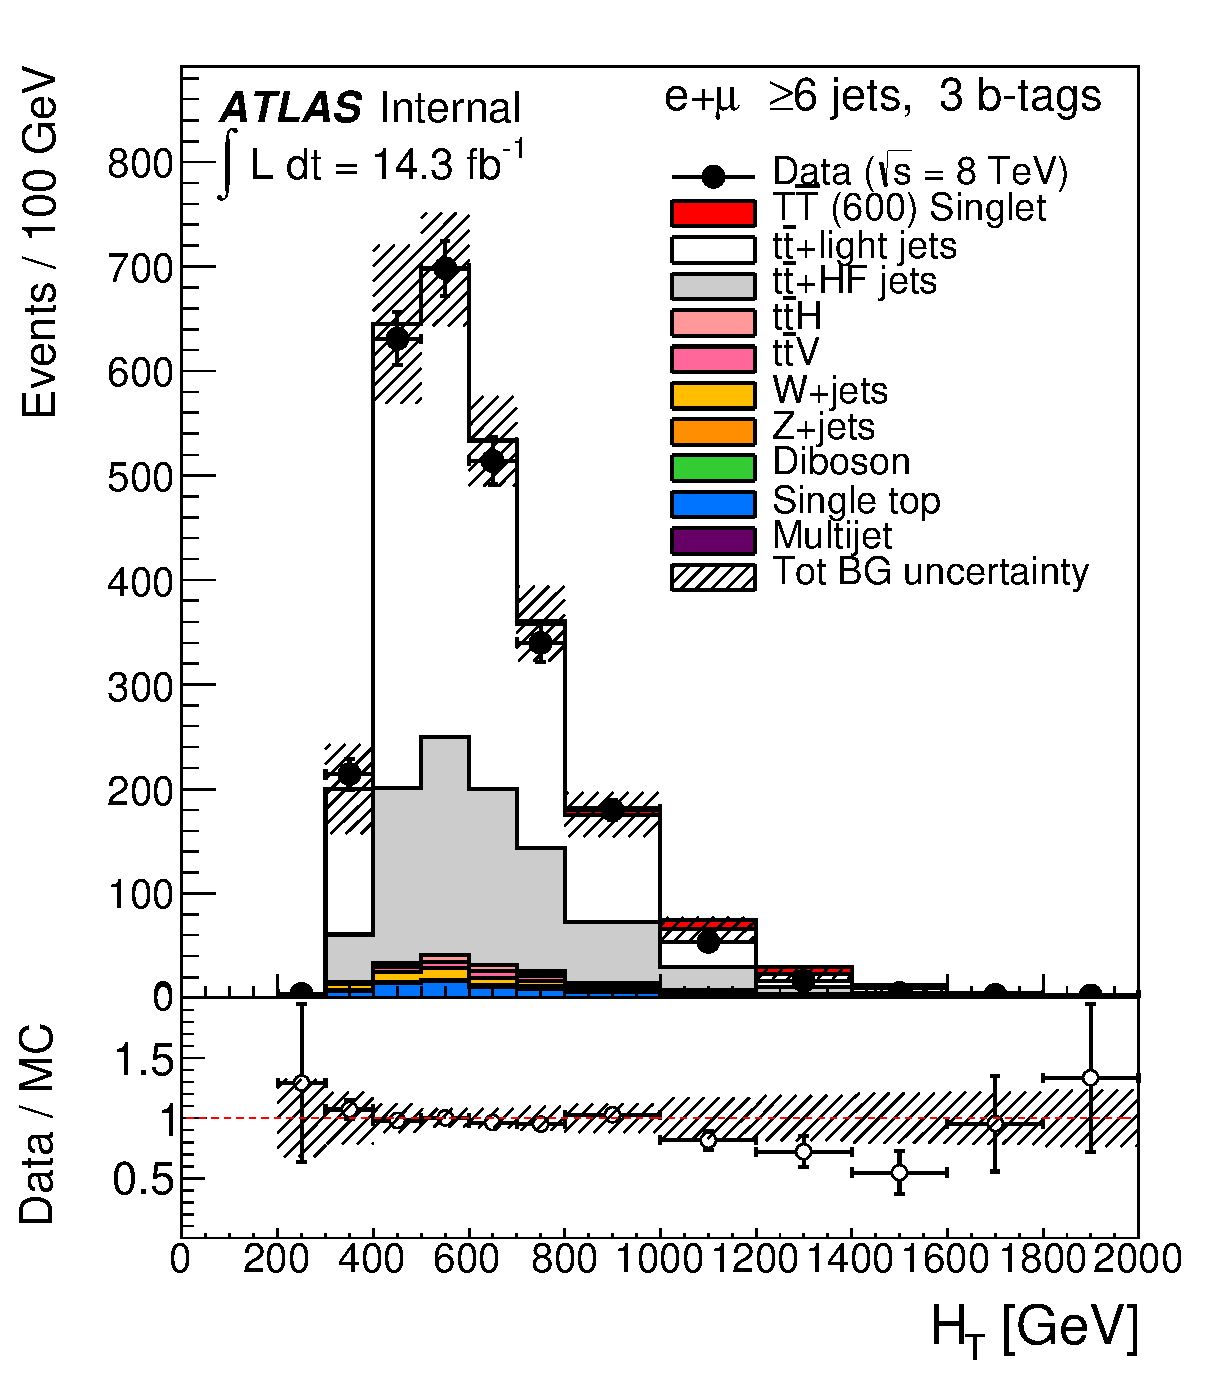
\includegraphics[width=0.45\textwidth]{results/figures/THESIS_c8_signal/HTAll_6jetin3btagex_ELEMUON.eps}}
	\subfigure[]{\label{fig:htx4}
%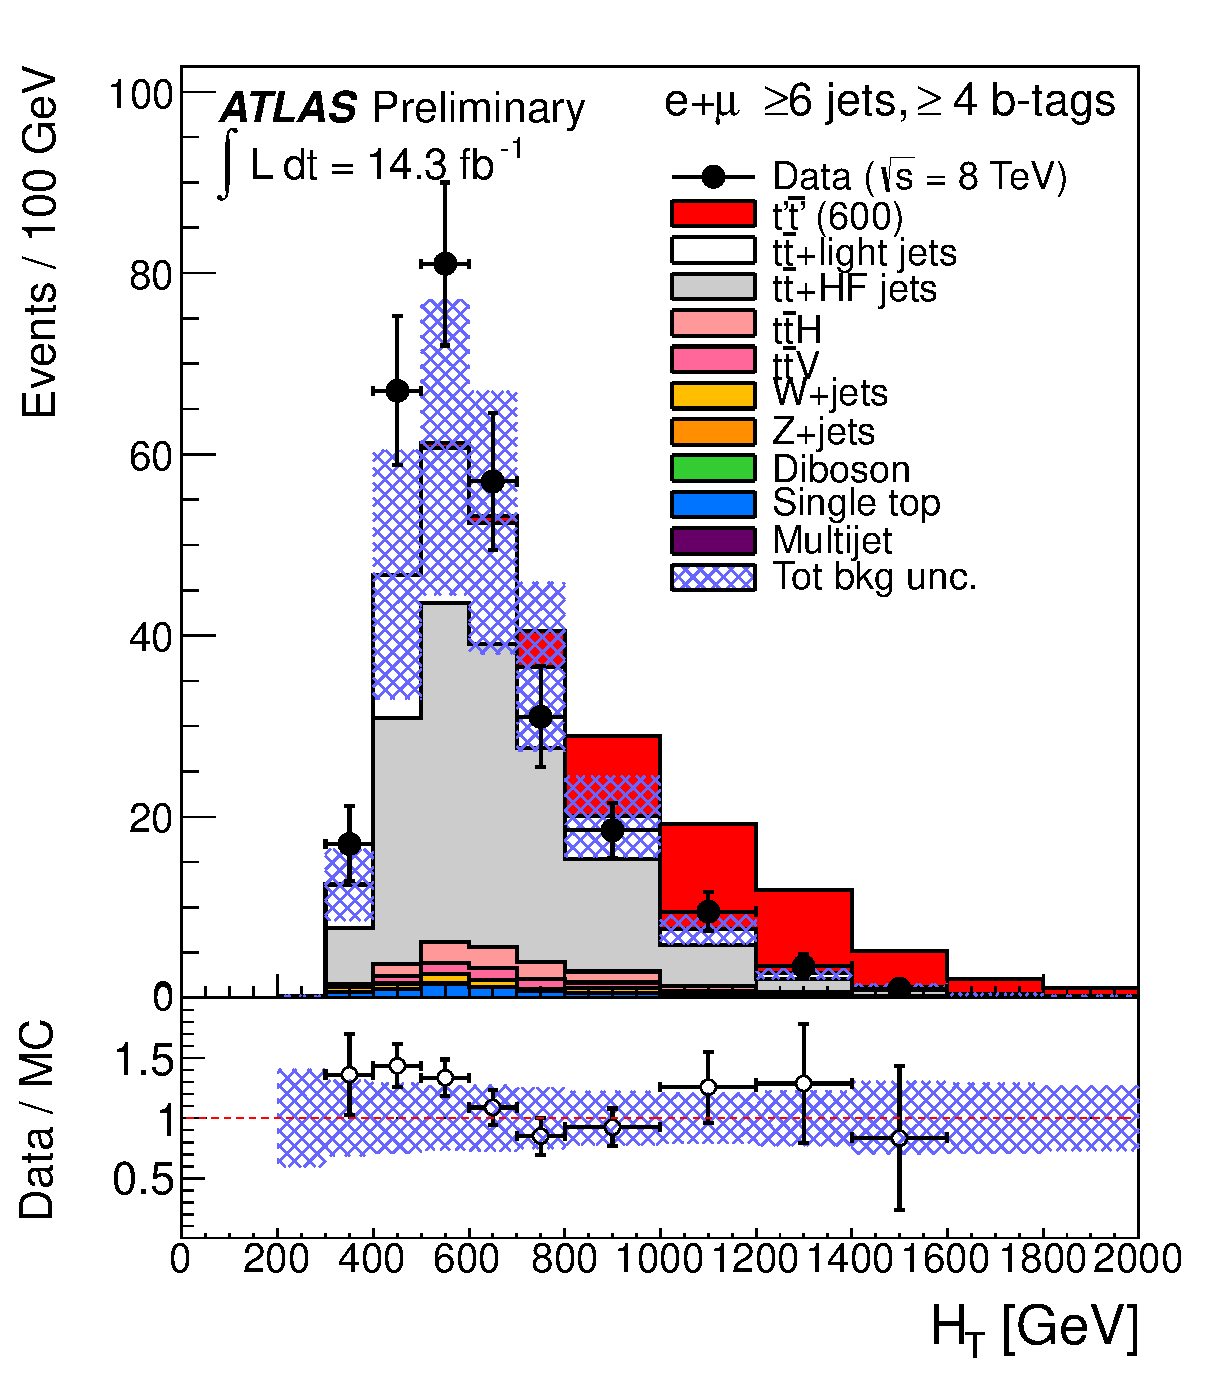
\includegraphics[width=0.45\textwidth]{htx_analysis_14ifb/figures/final/HTAll_6jetin4btagin_ELEMUON.eps}}
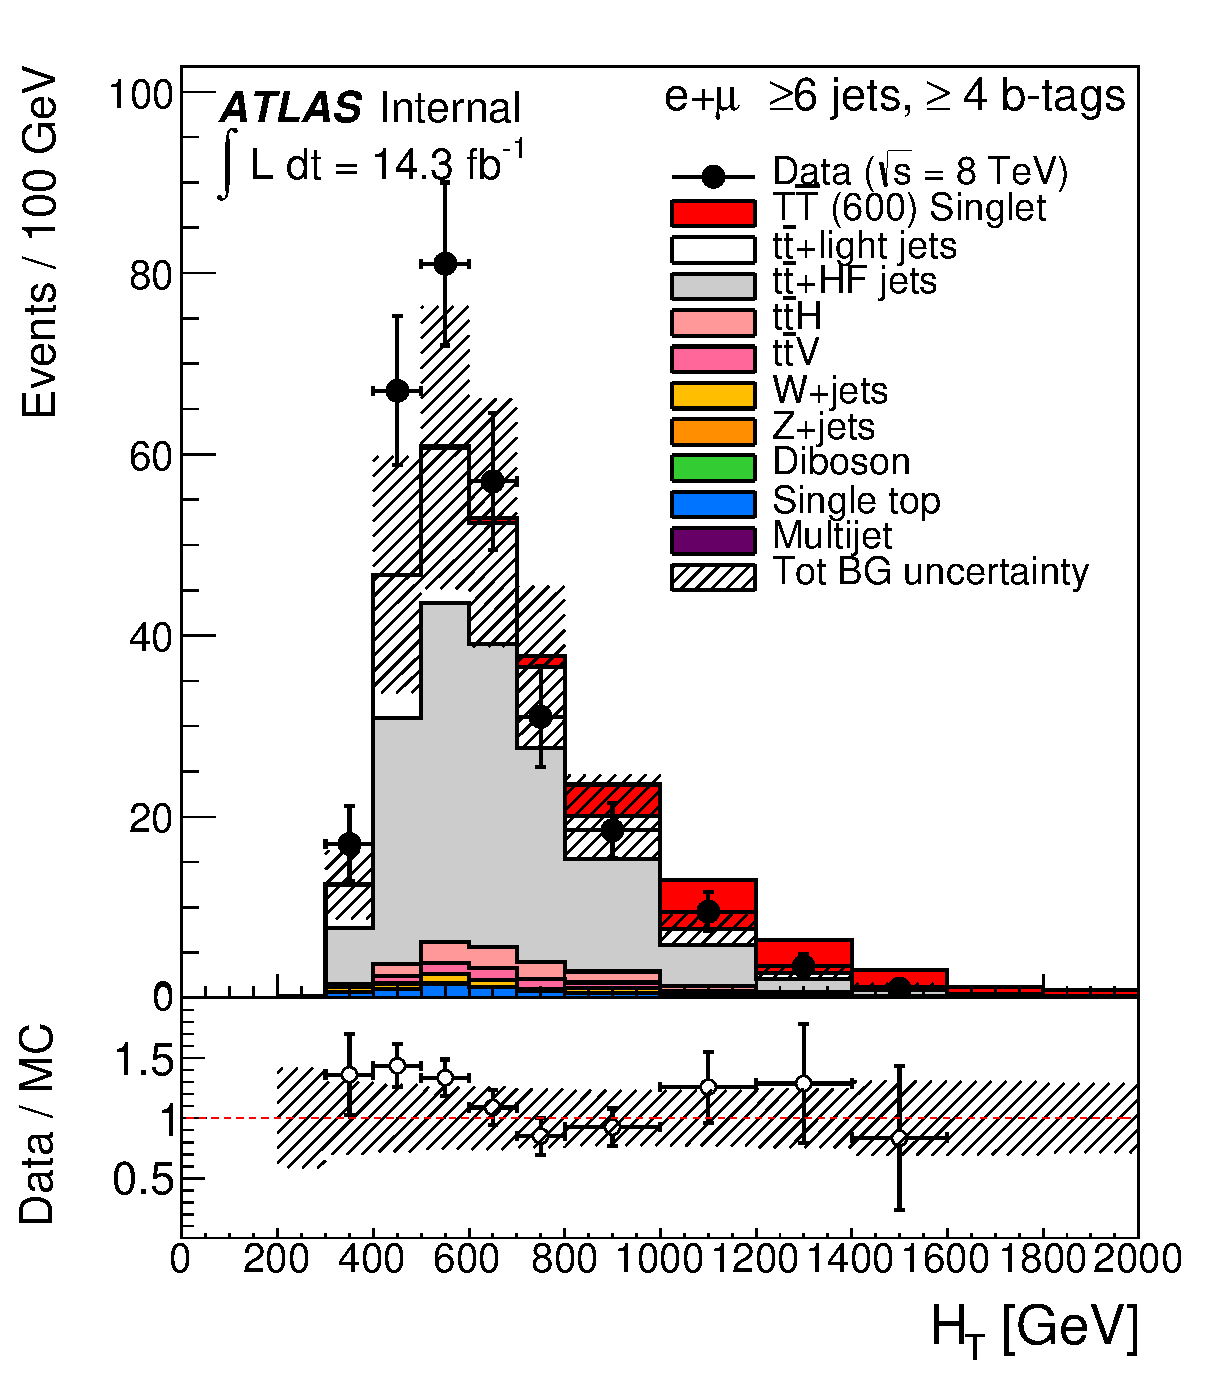
\includegraphics[width=0.45\textwidth]{results/figures/THESIS_c8_signal/HTAll_6jetin4btagin_ELEMUON.eps}}
	\subfigure[]{\label{fig:wbx1}
%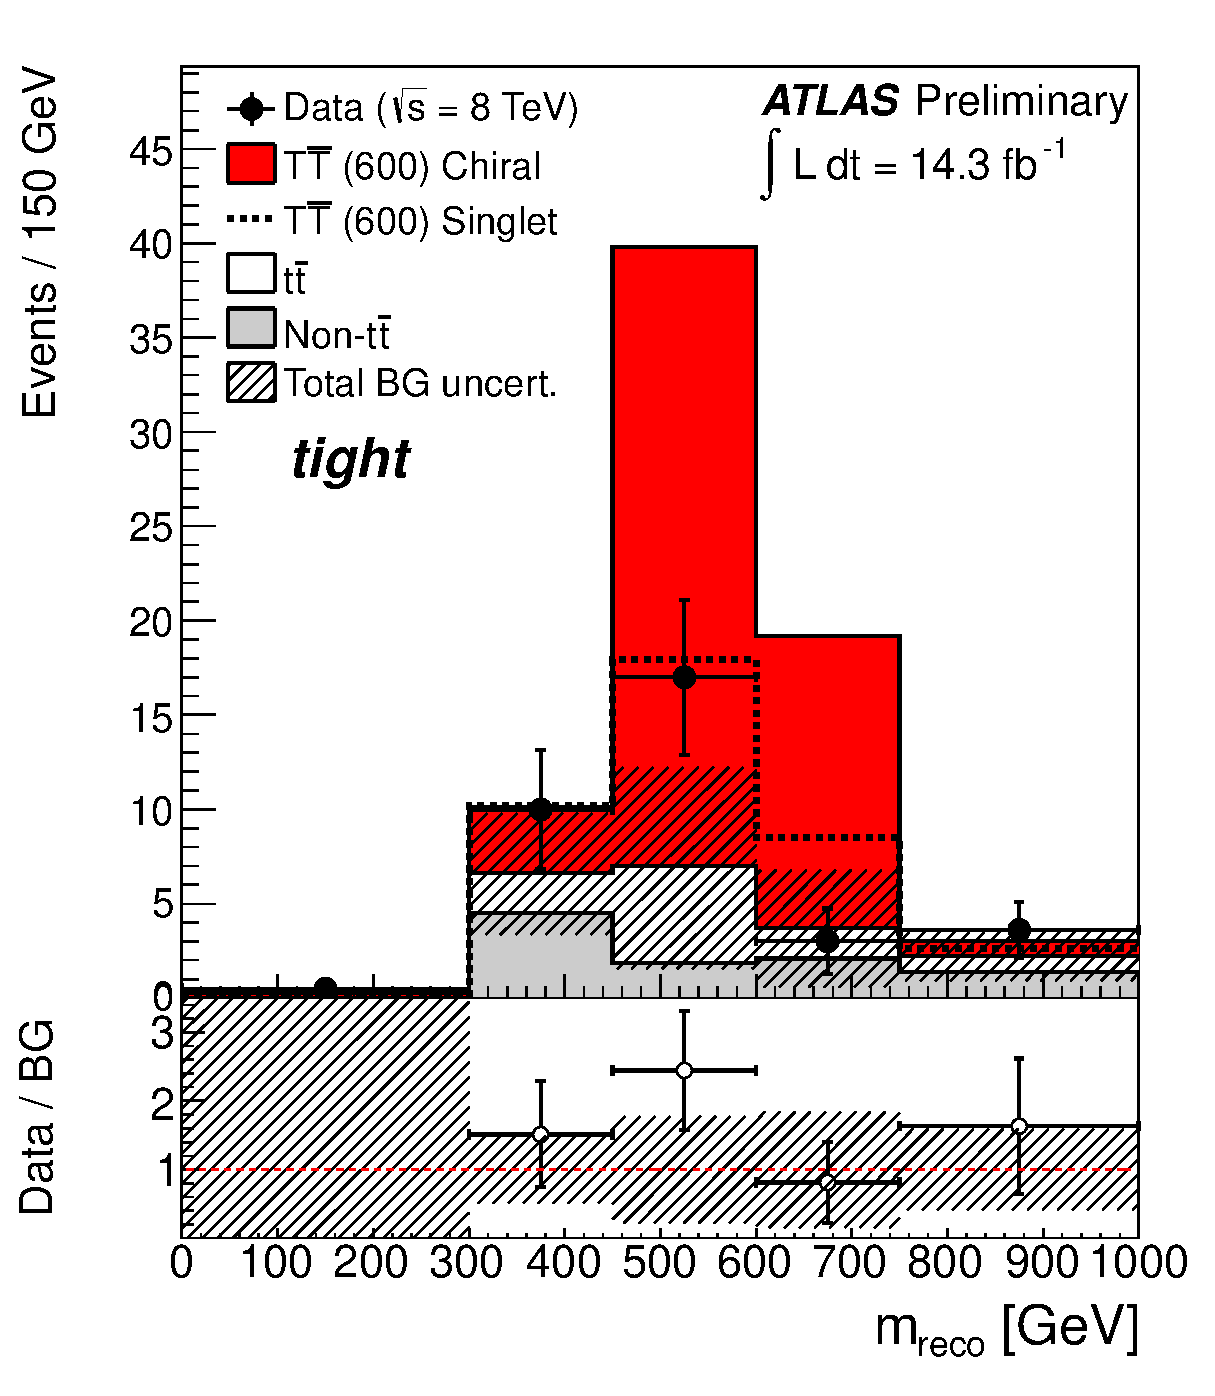
\includegraphics[width=0.45\textwidth]{wbx_analysis_14ifb/figures/confnoteplots/VLQAna_WbX_1W_MWb_4_ELEMUON_cutflow1234567_NOMINAL.eps}}
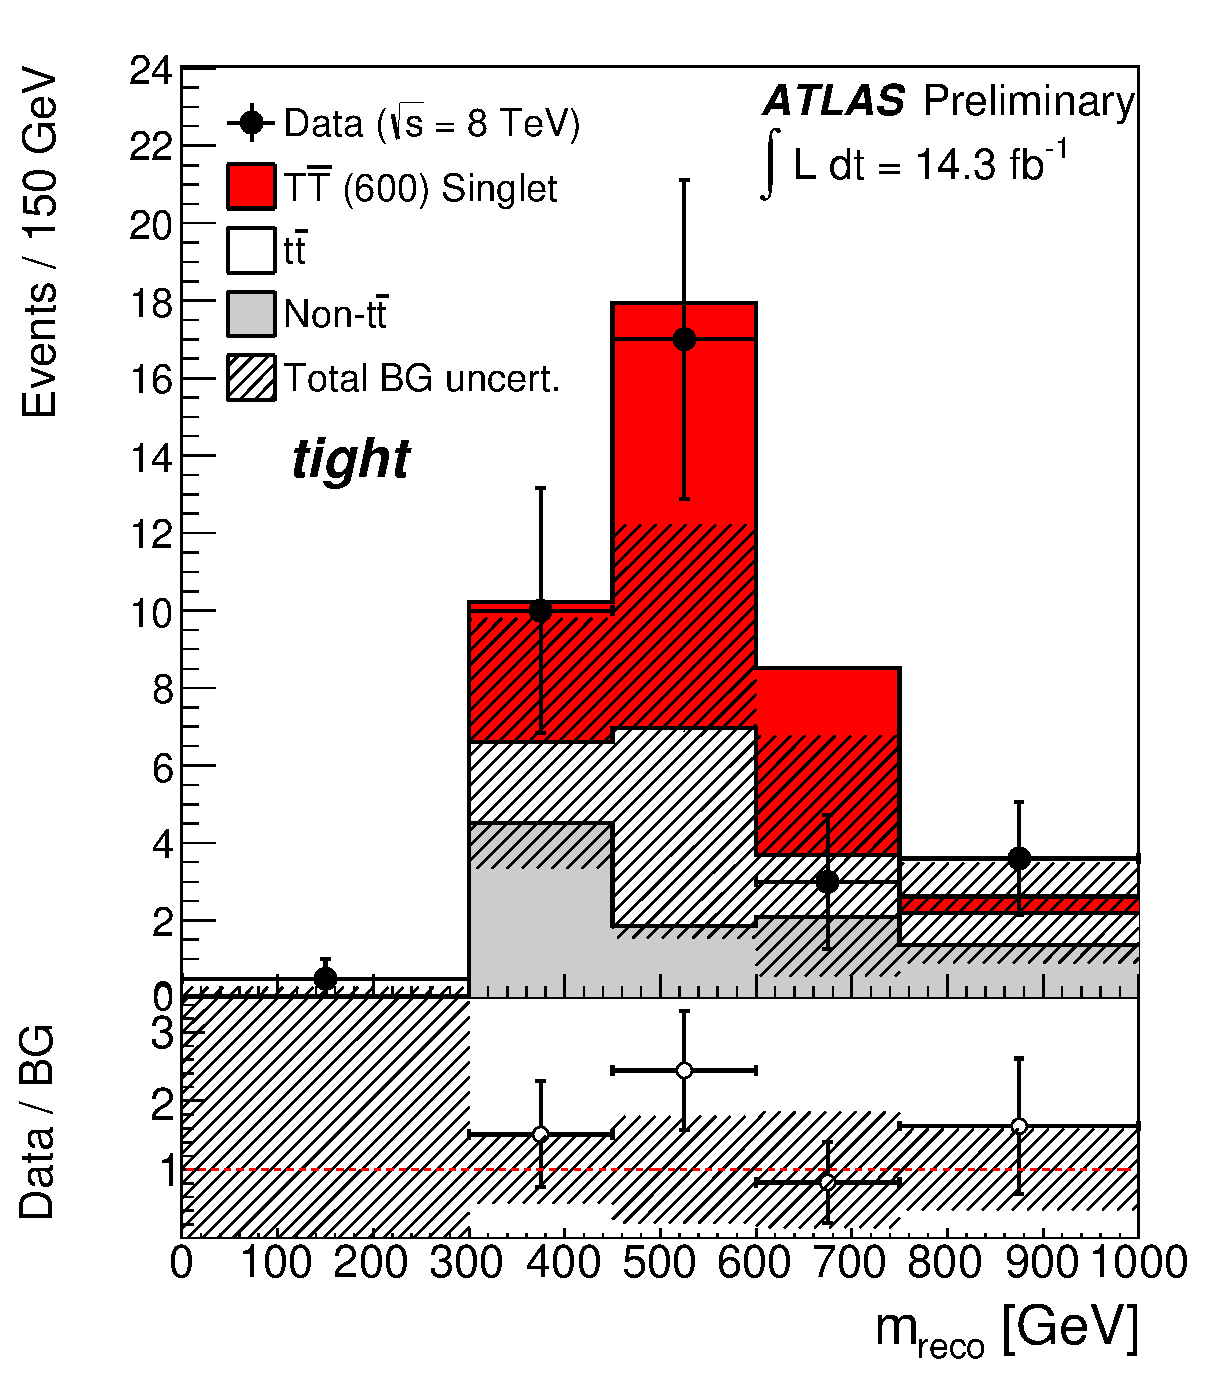
\includegraphics[width=0.45\textwidth]{results/figures/THESIS_c8_signal/VLQAna_WbX_1W_MWb_4_ELEMUON_cutflow1234567_NOMINAL.eps}}
	\caption{Final discriminant variables distributions in the search channels
        of the \htx\ analysis ($\HT$ in (a) \chii, (b) \chiii\ and (c) \chiv\ channels)
        and of the \wbx\ analysis (\mreco\ in the \tight\ channel). In all plots the
        signal is shown for the singlet model. The uncertainty bands include statistical 
        and systematic uncertainties.\label{fig:searchchan}}
\end{center}\end{figure}

For the purpose of a combined statistical analysis
of the four channels,
choices on the systematic 
uncertainties treatment have to be done.
Uncertainties that are common to both analyses and that
are treated in the same way are considered as fully 
correlated and are: integrated luminosity; lepton reconstruction, 
identification and trigger (1 component); jet vertex fraction;
jet energy resolution;
$b$ tagging (9 components); $c$ tagging (5 components); light-jet 
tagging (1 component);
background cross sections ($t\bar{t}$, single top, diboson, $t\bar{t}V$).
For the JES uncertainty, while the \wbx\ analysis considers a single component
the \htx\ uses the 8 components breakdown and is then impossible to 
correlate the individual JES uncertainty sources one by one.
Since in the \htx\ analysis the dominant JES uncertainty eigenvector is the BASELINE
(see Section~\ref{sec:htxSYS}) the choice is to correlate the \wbx\ analysis JES 
uncertainty with the BASELINE uncertainty of the \htx\ analysis.
The systematic uncertainties that are not taken as correlated are:
$W$+jets normalization, divided into 5 components in the \wbx\ 
analysis and only 1 in the \htx\ analysis where, however, is a negligible 
background; $t\bar{t}$ modeling, as the two analyses use different $t\bar{t}$ 
Monte Carlo generators and probe very different
final state kinematics region with different flavor composition.

The benchmark model chosen to show the exclusion limit as a function
of the mass is the vector-like singlet $T$ quark scenario, as
it is the common benchmark model for the two analyses. In this
case the \htx\ analysis performed better than the \wbx\ analysis,
giving an  observed (expected) 95\%  CL  limit value of
$m_{\T}>640\,(615)\gev$.
Figure~\ref{fig:limits1D_combo} shows the observed and expected 
upper limits on the \TTbar\ production cross section 
times branching fraction as a function of $m_{\T}$ for a weak-isospin
singlet  after combination of the two analyses.
The observed (expected) 95\% CL limit is 
$m_{\T}>670\,(675)\gev$ for the central value 
of the theoretical cross section,
improving by $\sim$30$\gev$ the expected sensitivity 
obtained by the \htx\ analysis alone.

\begin{figure}[h!tb]
\centering
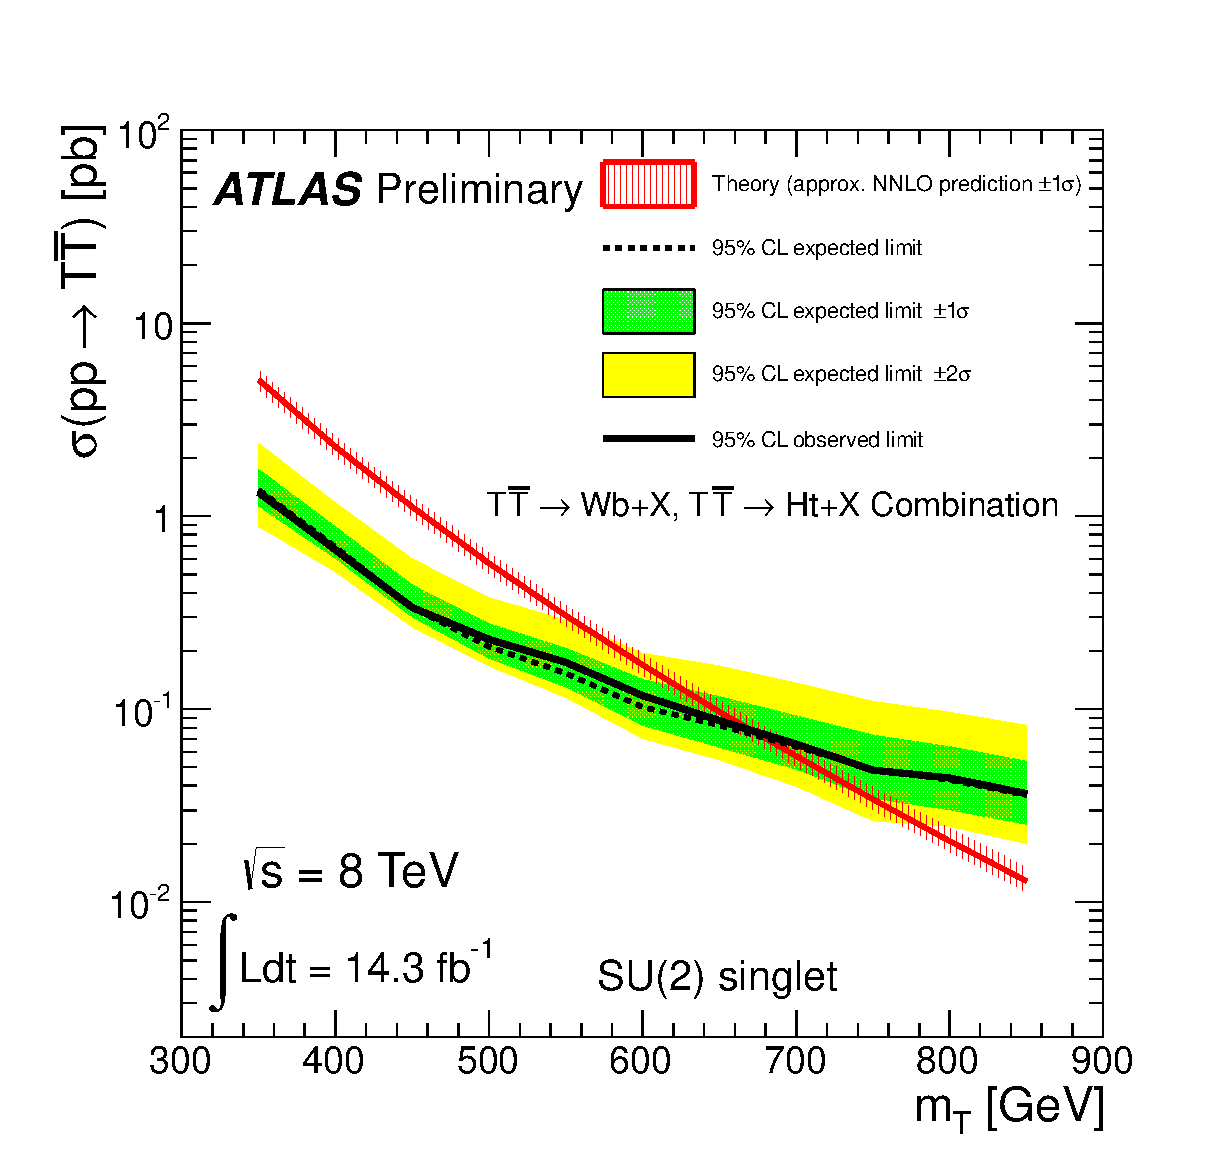
\includegraphics[width=0.45\textwidth]{results/figures/lim_singlet_comb.eps} 
\caption[bla]{Observed (solid line) and expected (dashed line) 95\% CL upper limit on the $\T \bar{\T}$ cross section times branching fraction
for a vector-like singlet $\T$ quark  as a function of the $\T$ quark mass, resulting from the combination of
the \wbx\ and the \htx\ analyses.
The surrounding shaded bands correspond to the $\pm1$ and $\pm2$ standard deviations around the expected limit. 
The thin red line and band show the theoretical prediction and its $\pm1$ standard deviation uncertainty.

\label{fig:limits1D_combo}}
\end{figure}

Figure~\ref{fig:limits2D_combo} shows the two-dimensional BR plane for 
different values of $m_{\T}$ with the  resulting 95\% CL exclusion limits.
Comparing this result with the ones of Figures~\ref{fig:limits2D_wbx} 
and~\ref{fig:limits2D_htx} it is evident the improvement resulting
from the combination of the two analyses, covering a much larger
area than the simple addition of two individual ones.
From this picture, vector-like top partners are completely excluded
no matter of the model in the mass range from 350~\gev\ up to 550~\gev\ 
(almost up to 600~\gev).

\begin{figure}[h!bt]
\centering
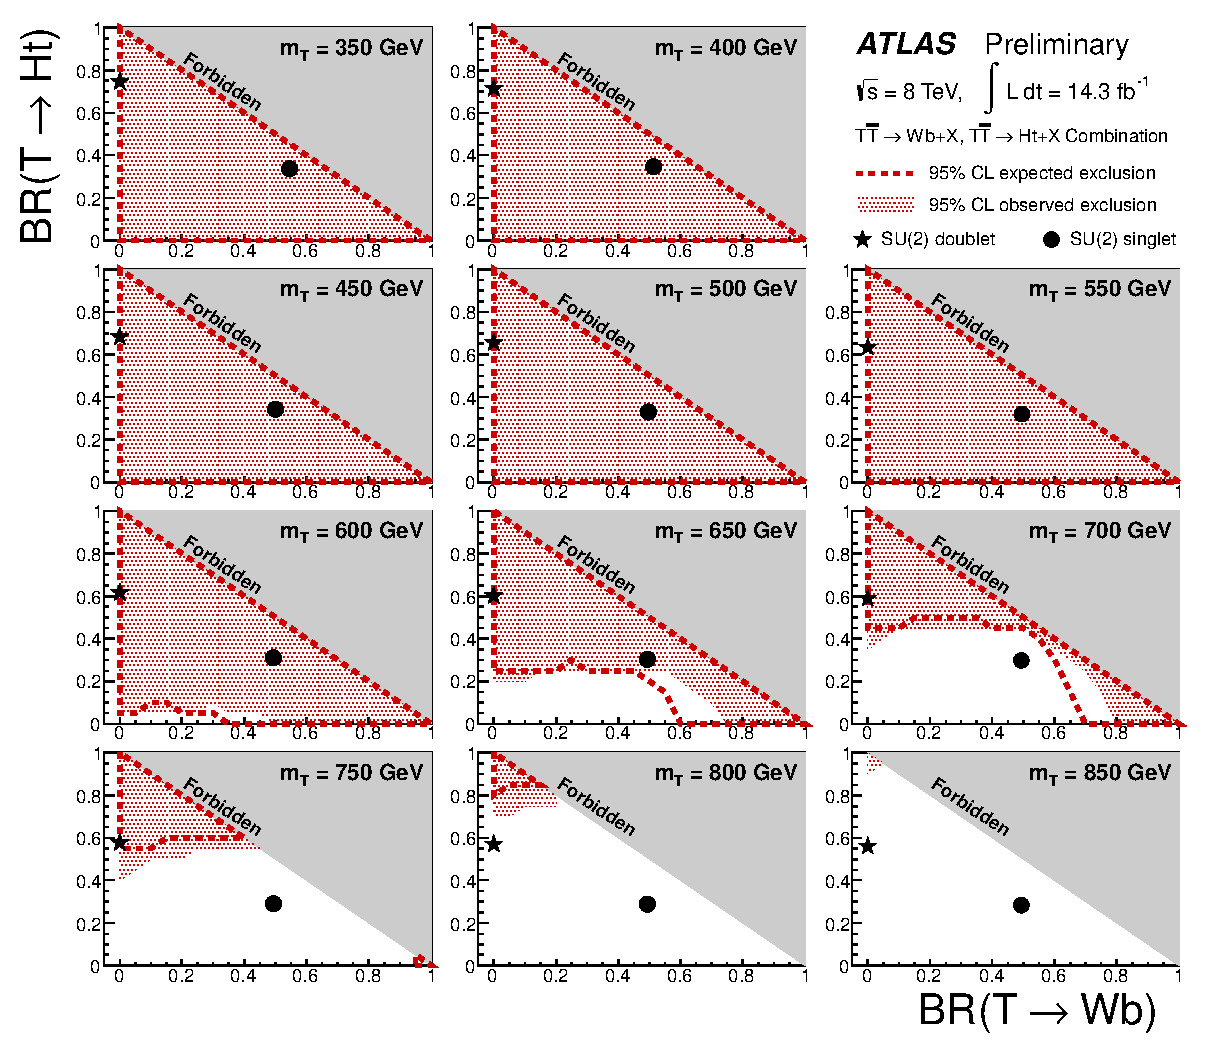
\includegraphics[width=0.9\textwidth]{results/figures/lim_Scan2D_comb.eps}
\caption{
Observed (red filled area) and expected (red dashed line) 95\% CL exclusion in the plane of
$BR(\T \to Wb)$ versus $BR(\T \to Ht)$, for different values of the vector-like $\T$ quark mass.
The grey (dark shaded) area corresponds to the unphysical region where the sum of branching ratios exceeds unity. 
The default branching ratio values from the \texttt{PROTOS} event generator for the weak-isospin singlet and doublet cases 
are shown as plain circle and star symbols, respectively. This result  from the combination of
the \wbx\ and \htx\ analyses includes both statistical and systematic uncertainties.
\label{fig:limits2D_combo}}
\end{figure}

It is interesting to compare the 
combined result
of the \wbx\ and \htx\ analyses
of Figure~\ref{fig:limits2D_combo} 
with the separate analysis results
to understand the impact on sensitivity
of the statistical combination of
the search channels.
This comparison is presented in 
Figure~\ref{fig:limits2D_potentialcombo},
where the combined result is overlapped
to the two separate results in the BR
plane.
Looking e.g. at the 650~\gev\ mass point,
it can be clearly seen how the singlet
scenario, lying outside of the expected exclusion
region in the case of the single \htx\ analysis,
is then swallowed in the exluded area when
the same analysis is combined with the
\wbx\ analysis, which alone does not even
reach the proximities of that benchmark point.


\begin{figure}[h!bt]
\centering
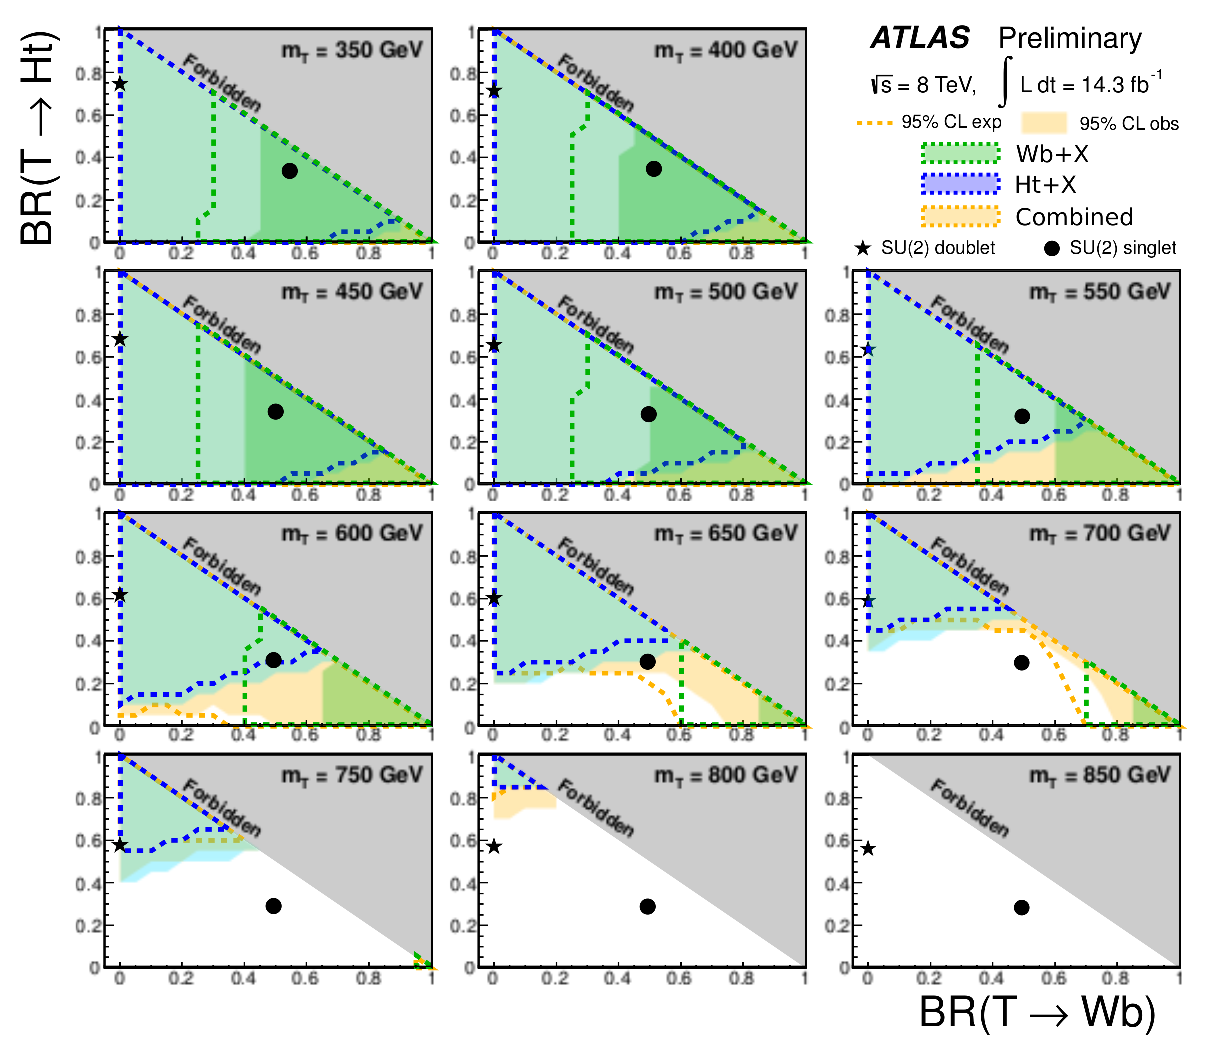
\includegraphics[width=0.9\textwidth]{results/figures/combinationoverlap.eps}
\caption{
Observed (filled area) and expected (dashed line) 95\% CL exclusion in the plane of
$BR(\T \to Wb)$ versus $BR(\T \to Ht)$, for different values of the $\T$ quark mass,
as result of the \wbx\ analysis (green), \htx\ analysis (blue), and the combination of the two (yellow).
The grey (dark shaded) area corresponds to the unphysical region where the sum of branching ratios exceeds unity. 
The default branching ratio values from the \texttt{PROTOS} event generator for the weak-isospin singlet and doublet cases 
are shown as plain circle and star symbols, respectively. All results
include both statistical and systematic uncertainties.
\label{fig:limits2D_potentialcombo}}
\end{figure}

\section{Comparison to other searches}\label{sec:coverage}

As briefly introduced in Section~\ref{sec:strategy}, two
additional analyses have been performed on the same dataset
as the \wbx\ and \htx\ analyses to search for heavy vector-like
top and bottom quarks in final states with exactly two leptons:
a search in the same-sign 
dilepton channel~\cite{ATLAS-CONF-2013-051} and 
a search in the opposite-charge dilepton channel~\cite{ATLAS-CONF-2013-056}.
It was shown that the four analyses probe different 
regions of the 2-dimensional mixing plane and are,
hence, complementary. Even though the single lepton and
the dilepton channels can be considered enough
separated, it was not possible to ensure a complete
orthogonality between all the analyses and they have
not, therefore, been combined\footnote{This
fact is mainly due to the different timescales
and frameworks at which the analyses have been developed. 
The \wbx\ and \htx\ searches
have been conceived to be combined since the
early stages of their design and were performed
inside the same analysis framework.}.
It is however useful to visualize how
the four searches contribute to the full
coverage of the BRs mixing plane by
observing Figure~\ref{fig:limits2D_allcombo}.
Here the results from the four searches,
each obtained independentely, are simply
overlapped. This picture corresponds somehow to
a ``worst case scenario'' of a possible
real combination of the four searches, as
in general the statistical analysis in the
case of additional signal enriched
channels would gain sensitivity. 
This can easily be grasped when looking
at the comparison between the combined result
of the \wbx\ and \htx\ analyses
with the plain overlap of the separate
coverages, shown in the previous section 
in Figure~\ref{fig:limits2D_potentialcombo}.

Figure~\ref{fig:limits2D_allcombo} shows that already
without combining any of the four searches,
\T\ quarks with masses up to 550~\gev, almost up
to 600~\gev, are excluded at 95\% CL without 
any assumption on the model. The same kind of
picture has been obtained in the BR plane for
\B\ quarks, shown in Figure~\ref{fig:limits2D_allvlb}.
Here the analyses contributing to the
95\% CL exclusion in the BR($B\to Hb$) vs  BR($B\to Wt$)
plane are the two searches in the multilepton channel.
The absence of a search probing the top-left corner
of the BR plane leaves for \B\ masses from 400~\gev up to
600~\gev only a very small area uncovered.


\begin{landscape}
\begin{figure}[h!bt]
\centering
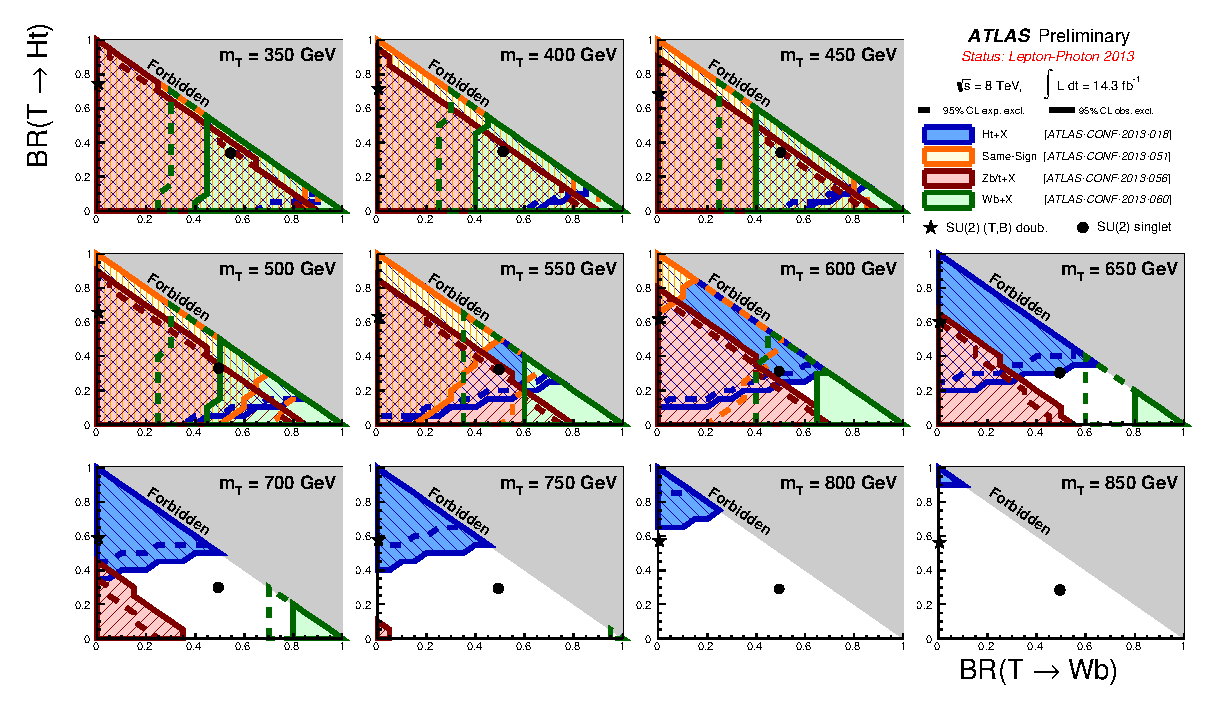
\includegraphics[width=1.5\textwidth]{results/figures/ATLAS_VLQ_TT_june2013_step4.eps}
\caption{
Observed (filled area) and expected (dashed line) 95\% CL exclusion in the plane of
$BR(\T \to Wb)$ versus $BR(\T \to Ht)$, for different values of the $\T$ quark mass.
In blue is shown the area excluded by the single lepton \htx\ analysis;
in orange is shown the area excluded by the same-sign dilepton analysis;
in red is shown the area excluded by the opposite-sign dilepton $\TTbar\to Zt+X$ analysis;
in green is shown the area excluded by the single lepton \wbx\ analysis.
The grey (dark shaded) area corresponds to the unphysical region where the sum of branching ratios exceeds unity. 
The default branching ratio values from the \texttt{PROTOS} event generator for the weak-isospin singlet and doublet cases 
are shown as plain circle and star symbols, respectively. This result includes both statistical and systematic uncertainties.
\label{fig:limits2D_allcombo}}
\end{figure}
\end{landscape}


\begin{landscape}
\begin{figure}[h!bt]
\centering
\includegraphics[width=1.5\textwidth]{results/figures/ATLAS_VLQ_BB_june2013_step2.eps}
\caption{
Observed (filled area) and expected (dashed line) 95\% CL exclusion in the plane of
$BR(\B \to Wt)$ versus $BR(\B \to Hb)$, for different values of the $\B$ quark mass.
In orange is shown the area excluded by the same-sign dilepton analysis;
in red is shown the area excluded by the opposite-sign dilepton $\TTbar\to Zt+X$ analysis.
The grey (dark shaded) area corresponds to the unphysical region where the sum of branching ratios exceeds unity. 
The default branching ratio values from the \texttt{PROTOS} event generator for the weak-isospin singlet and doublet cases 
are shown as plain circle and star symbols, respectively. This result includes both statistical and systematic uncertainties.
\label{fig:limits2D_allvlb}}
\end{figure}
\end{landscape}



\section{Outlook}\label{sec:combOUT}

At the time this dissertation is being
written, all of the four searches for
vector-like quarks are being updated to
the full available statistics of
pp collisions at \rts=8~\tev, about 20~\ifb,
for publication. The four searches maintain the
core strategies but have improvements in
background modeling (in particular with better
and more statistically populated Monte Carlo samples)
and reduced systematic uncertainties.
Searches in new channels are being developed, namely
$B\to Wt+X$ and $B\to Hb+X$, thus allowing for
the full coverage of the BR plane corners.
The complete plan for vector-like quark searches
in ATLAS is to combine all these analyses to 
achieve the highest sensitivity available.
